\section{Цель работы}
Освоение принципов построения систем адаптивного и робастного управления на примере задачи слежения выхода скалярного объекта за эталонным сигналом.

\section{Теоретические сведения}
Рассматриваемый объект управления:
\begin{equation}
    \dot{x} = \theta x + u + \delta,
\end{equation}
где $x$~--- переменная состояния объекта, $u$~--- сигнал управления, $\theta$~--- неизвестный постоянный параметр, $\delta$~--- ограниченное внешнее возмущение, удовлетворяющее неравенству $|\delta(t)| \le \overline{\delta}$.

Возмущающее воздействие $\delta(t)$ имеет вид:
\begin{equation}\label{eq_delta}
	\delta(t) = (1 + t)^{-\frac{1}{8}} \left[1 - \theta (1 + t)^{-\frac{1}{4}} - \frac{3}{8} (1 + t)^{-\frac{5}{4}}\right].
\end{equation}

Цель управления заключается построении такого закона управления, чтобы обеспечивалось неравенство :
\begin{equation}\label{eq_goal_of_control}
	|x_m(t) - x(t)| = |\varepsilon(t)| \le \overline{\Delta}, \forall{t} \ge T,
\end{equation}
где $\varepsilon = x_m - x$~--- ошибка управления, $x_m$~--- эталонный сигнал, являющийся выходом динамической модели вида (т.н. эталонной модели)
\begin{equation}
    \dot{x}_m = - \lambda x_m + \lambda g,
\end{equation}
где $g$~--- сигнал задания, $\lambda$~--- параметр, задающий желаемое время переходного процесса.

Для решение поставленной задачи используется настраиваемый регулятор:
\begin{equation}\label{eq_tuned_controller}
    u = -\hat{\theta} x - \lambda x + \lambda g
\end{equation}
совместно с тремя анализируемыми алгоритма адаптации:
\begin{enumerate}
	\item 	Алгоритм адаптации (АА), использованный для невозмущенного ОУ:
	\begin{equation}\label{eq_AA_1}
		\dot{\hat{\theta}} = -\gamma x \varepsilon,
	\end{equation}
	\item Модификация АА из п.1:
	\begin{equation}\label{eq_AA_2}
		{\hat{\theta}} = -\gamma x \varepsilon,
	\end{equation}
	\item АА из п.1 с обратной связью по величине настраиваемого параметра:
	\begin{equation}\label{eq_AA_3}
		\dot{\hat{\theta}} = - \sigma \hat{\theta} -\gamma x \varepsilon \ldotp
	\end{equation}
\end{enumerate}

\section{Исходные данные}
Варианту \textnumero2 соответствует следующий набор исходных данных:
\begin{equation}
    \theta = 2,
    \qquad
    \lambda = 2,
    \qquad
    g(t) = \cos 4t \ldotp
\end{equation}


\section{Результаты экспериментов}
См.~рисунки~\ref{img_first}--\ref{img_aa_3_s0.01} и подписи к ним.

\begin{figure}[h!]
    \centering
    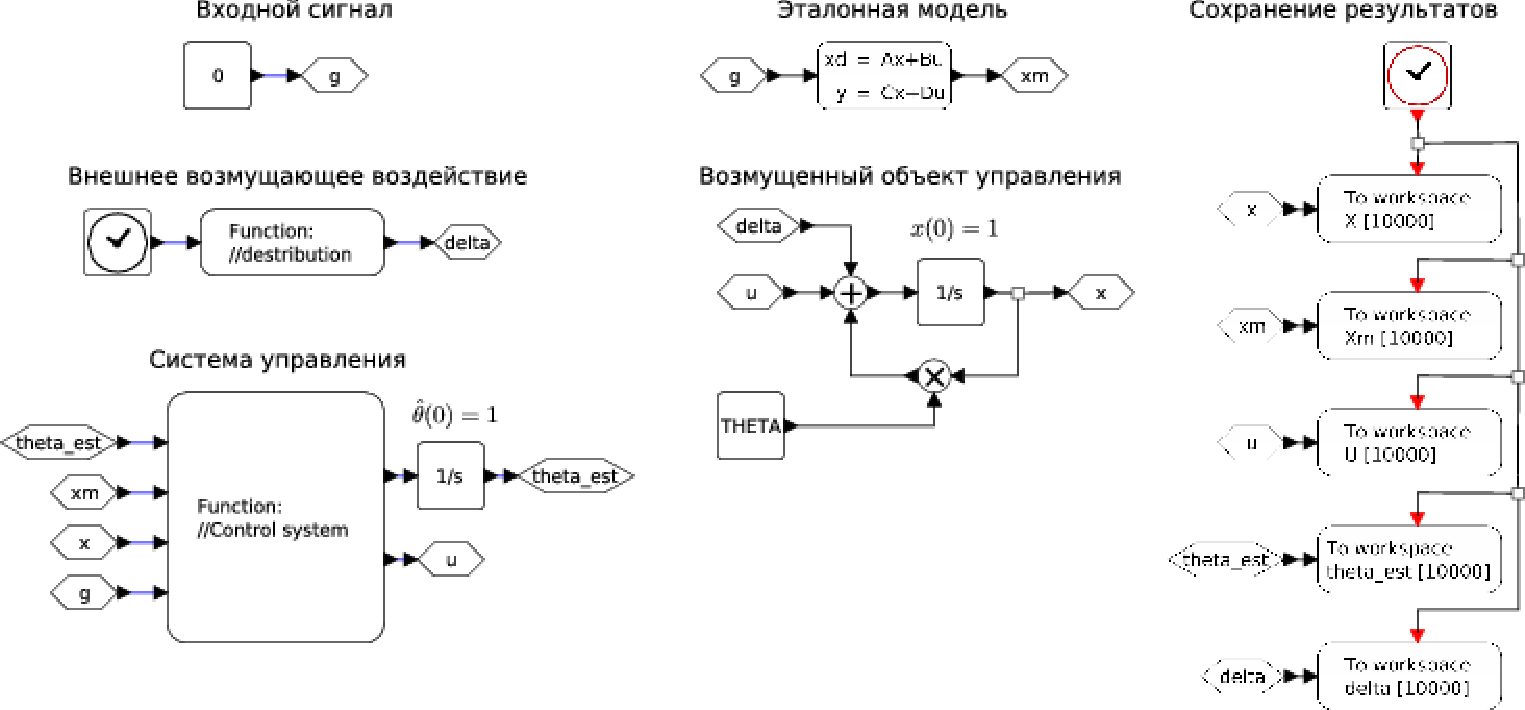
\includegraphics[width=\textwidth]{adapt_desturbance_model.pdf}
    \caption{Схема моделирования процесса управления с помощью настраиваемого регулятора из п.1 в условиях действия на ОУ возмущения~\ref{eq_delta}}
    \label{img_first}
\end{figure}

\begin{figure}[h!]
    \centering
    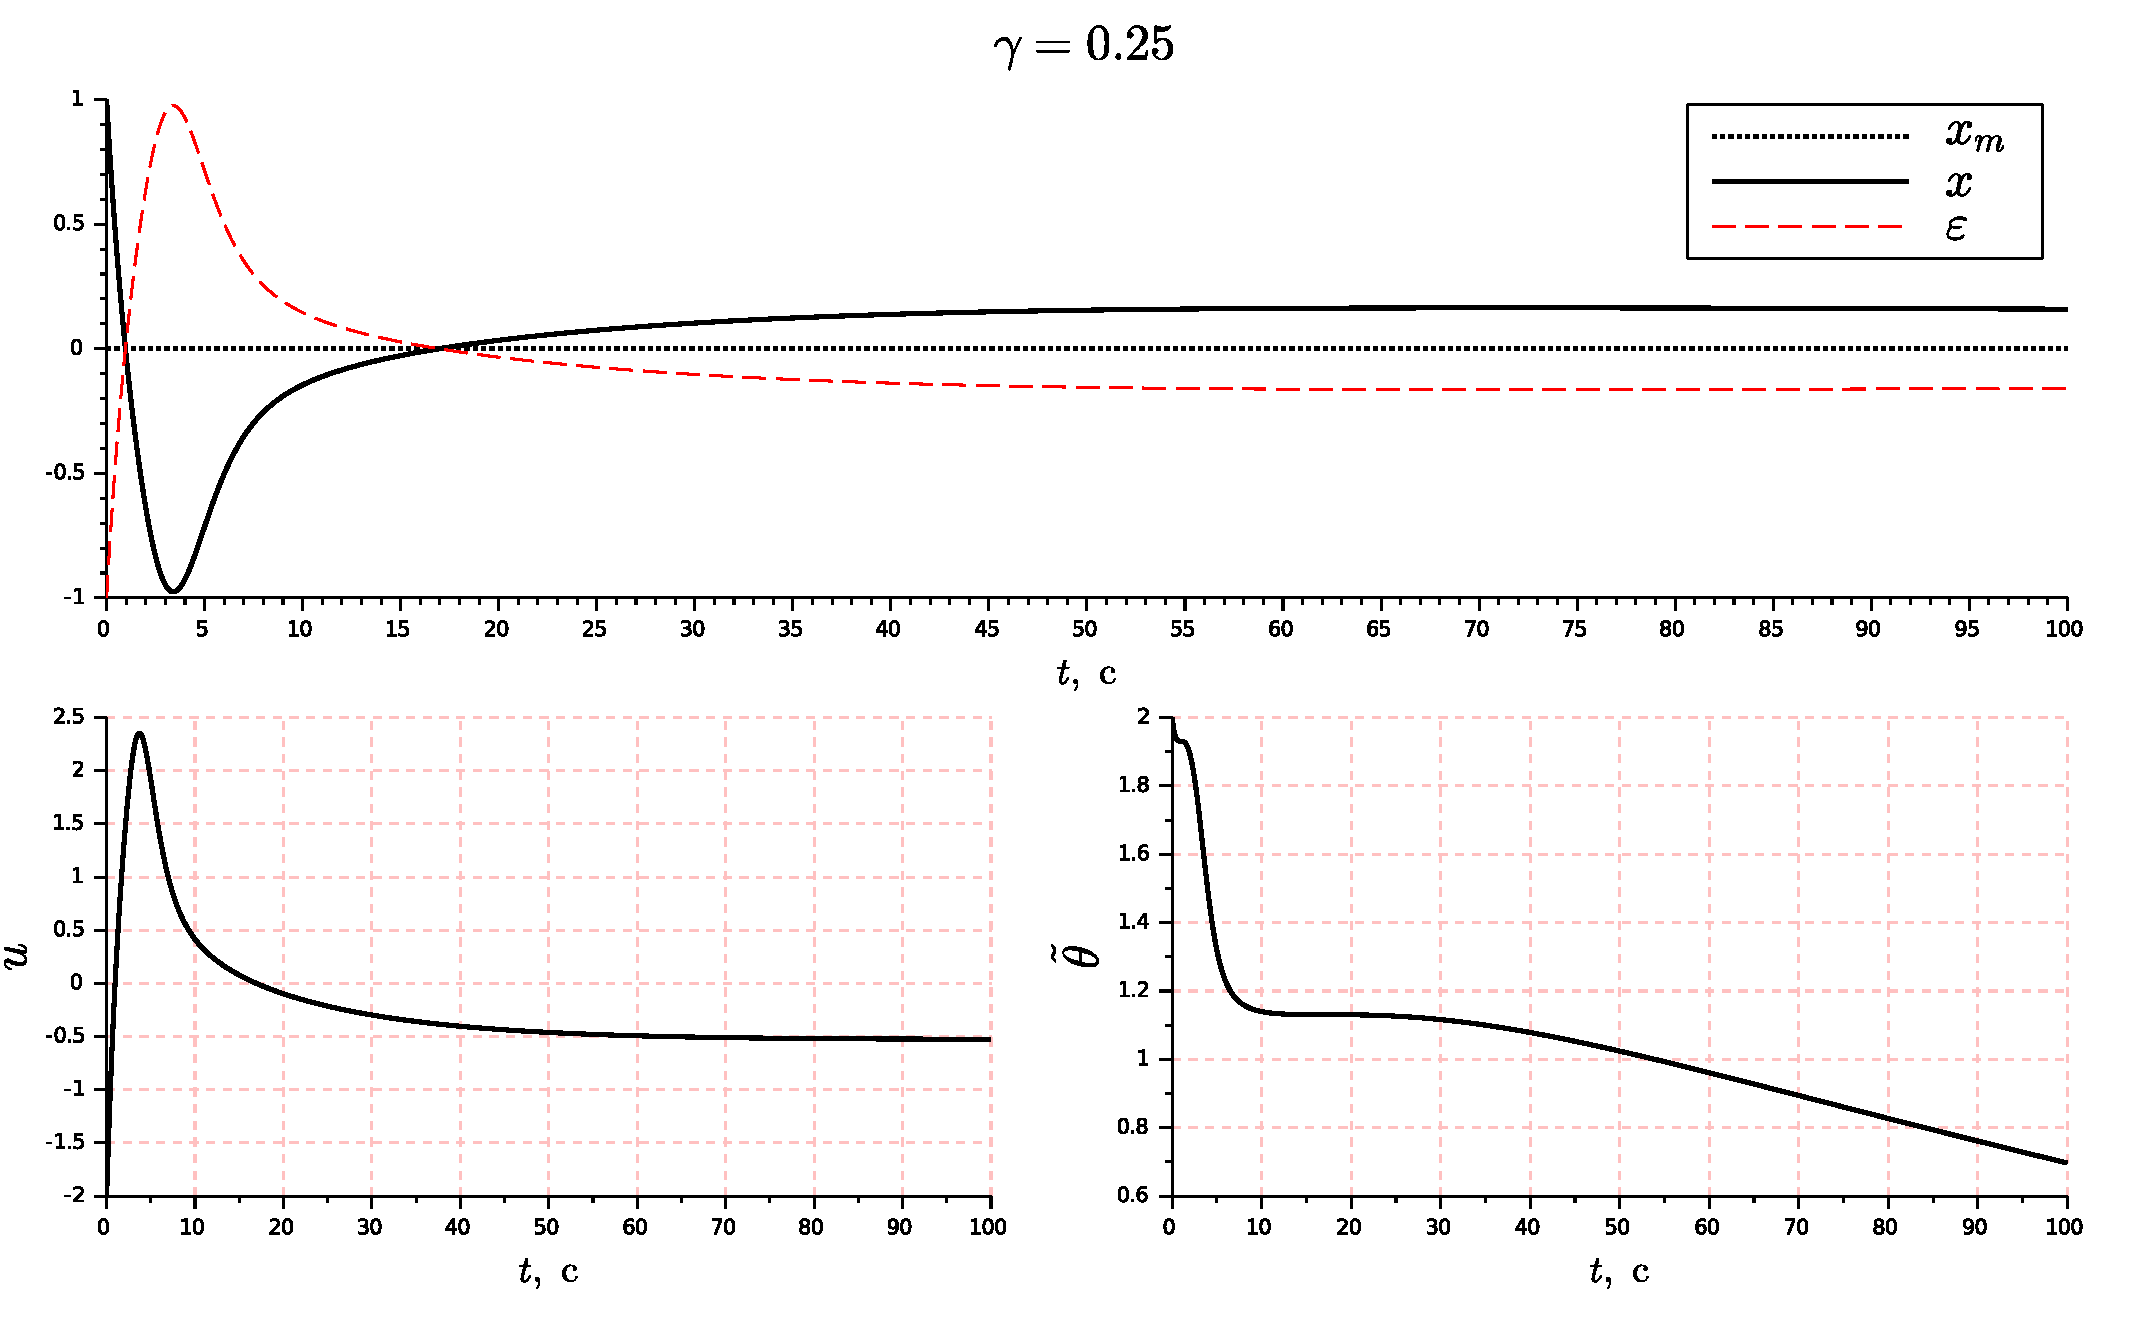
\includegraphics[width=\textwidth]{adapt_desturbance.pdf}
    \caption{Результаты моделирования процесса управления с помощью настраиваемого регулятора с АА из п.1}
    \label{img_aa_1}
\end{figure}

\begin{figure}[h!]
	\centering
	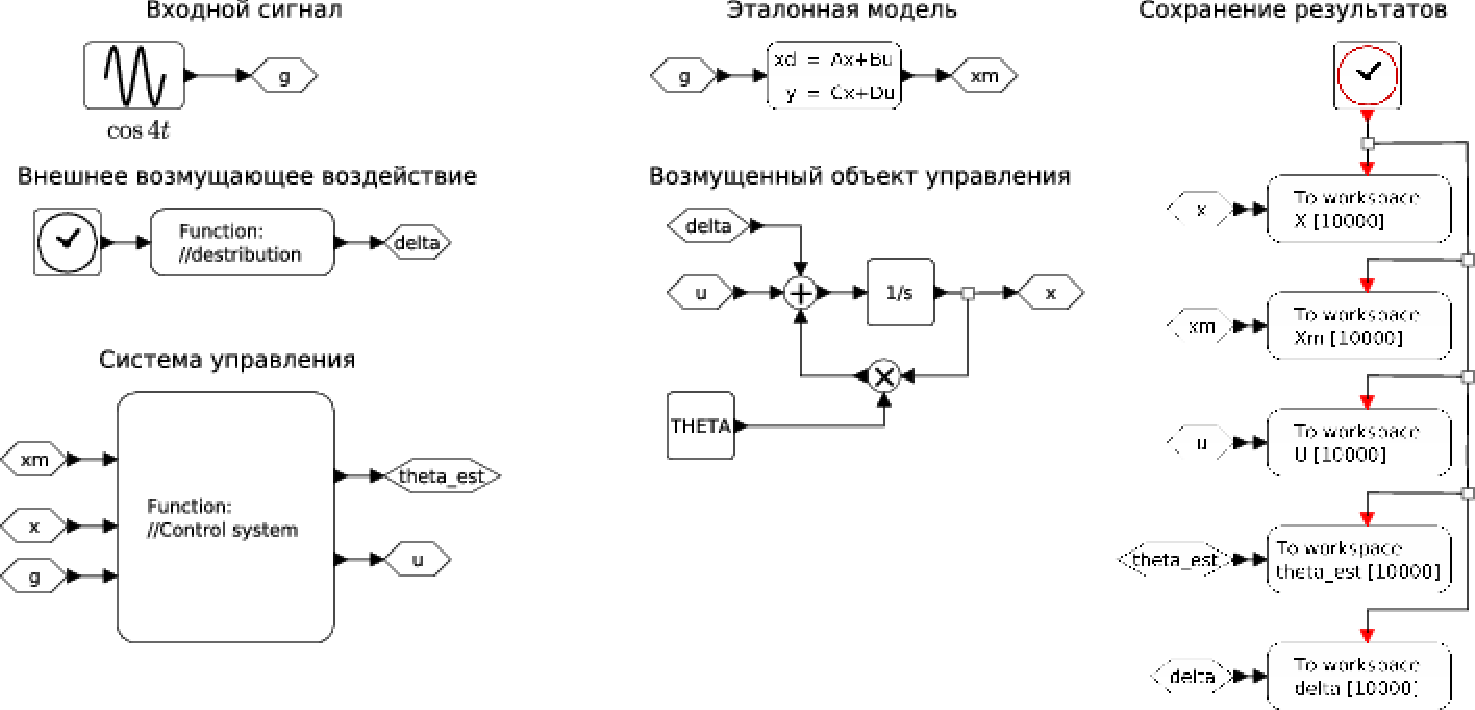
\includegraphics[width=\textwidth]{adapt_desturbance_model_solve_1.pdf}
	\caption{Схема моделирования процесса управления с помощью настраиваемого регулятора из п.2 в условиях действия на ОУ возмущения~\ref{eq_delta}}
	\label{img_schema_2}
\end{figure}

\begin{figure}[h!]
    \centering
    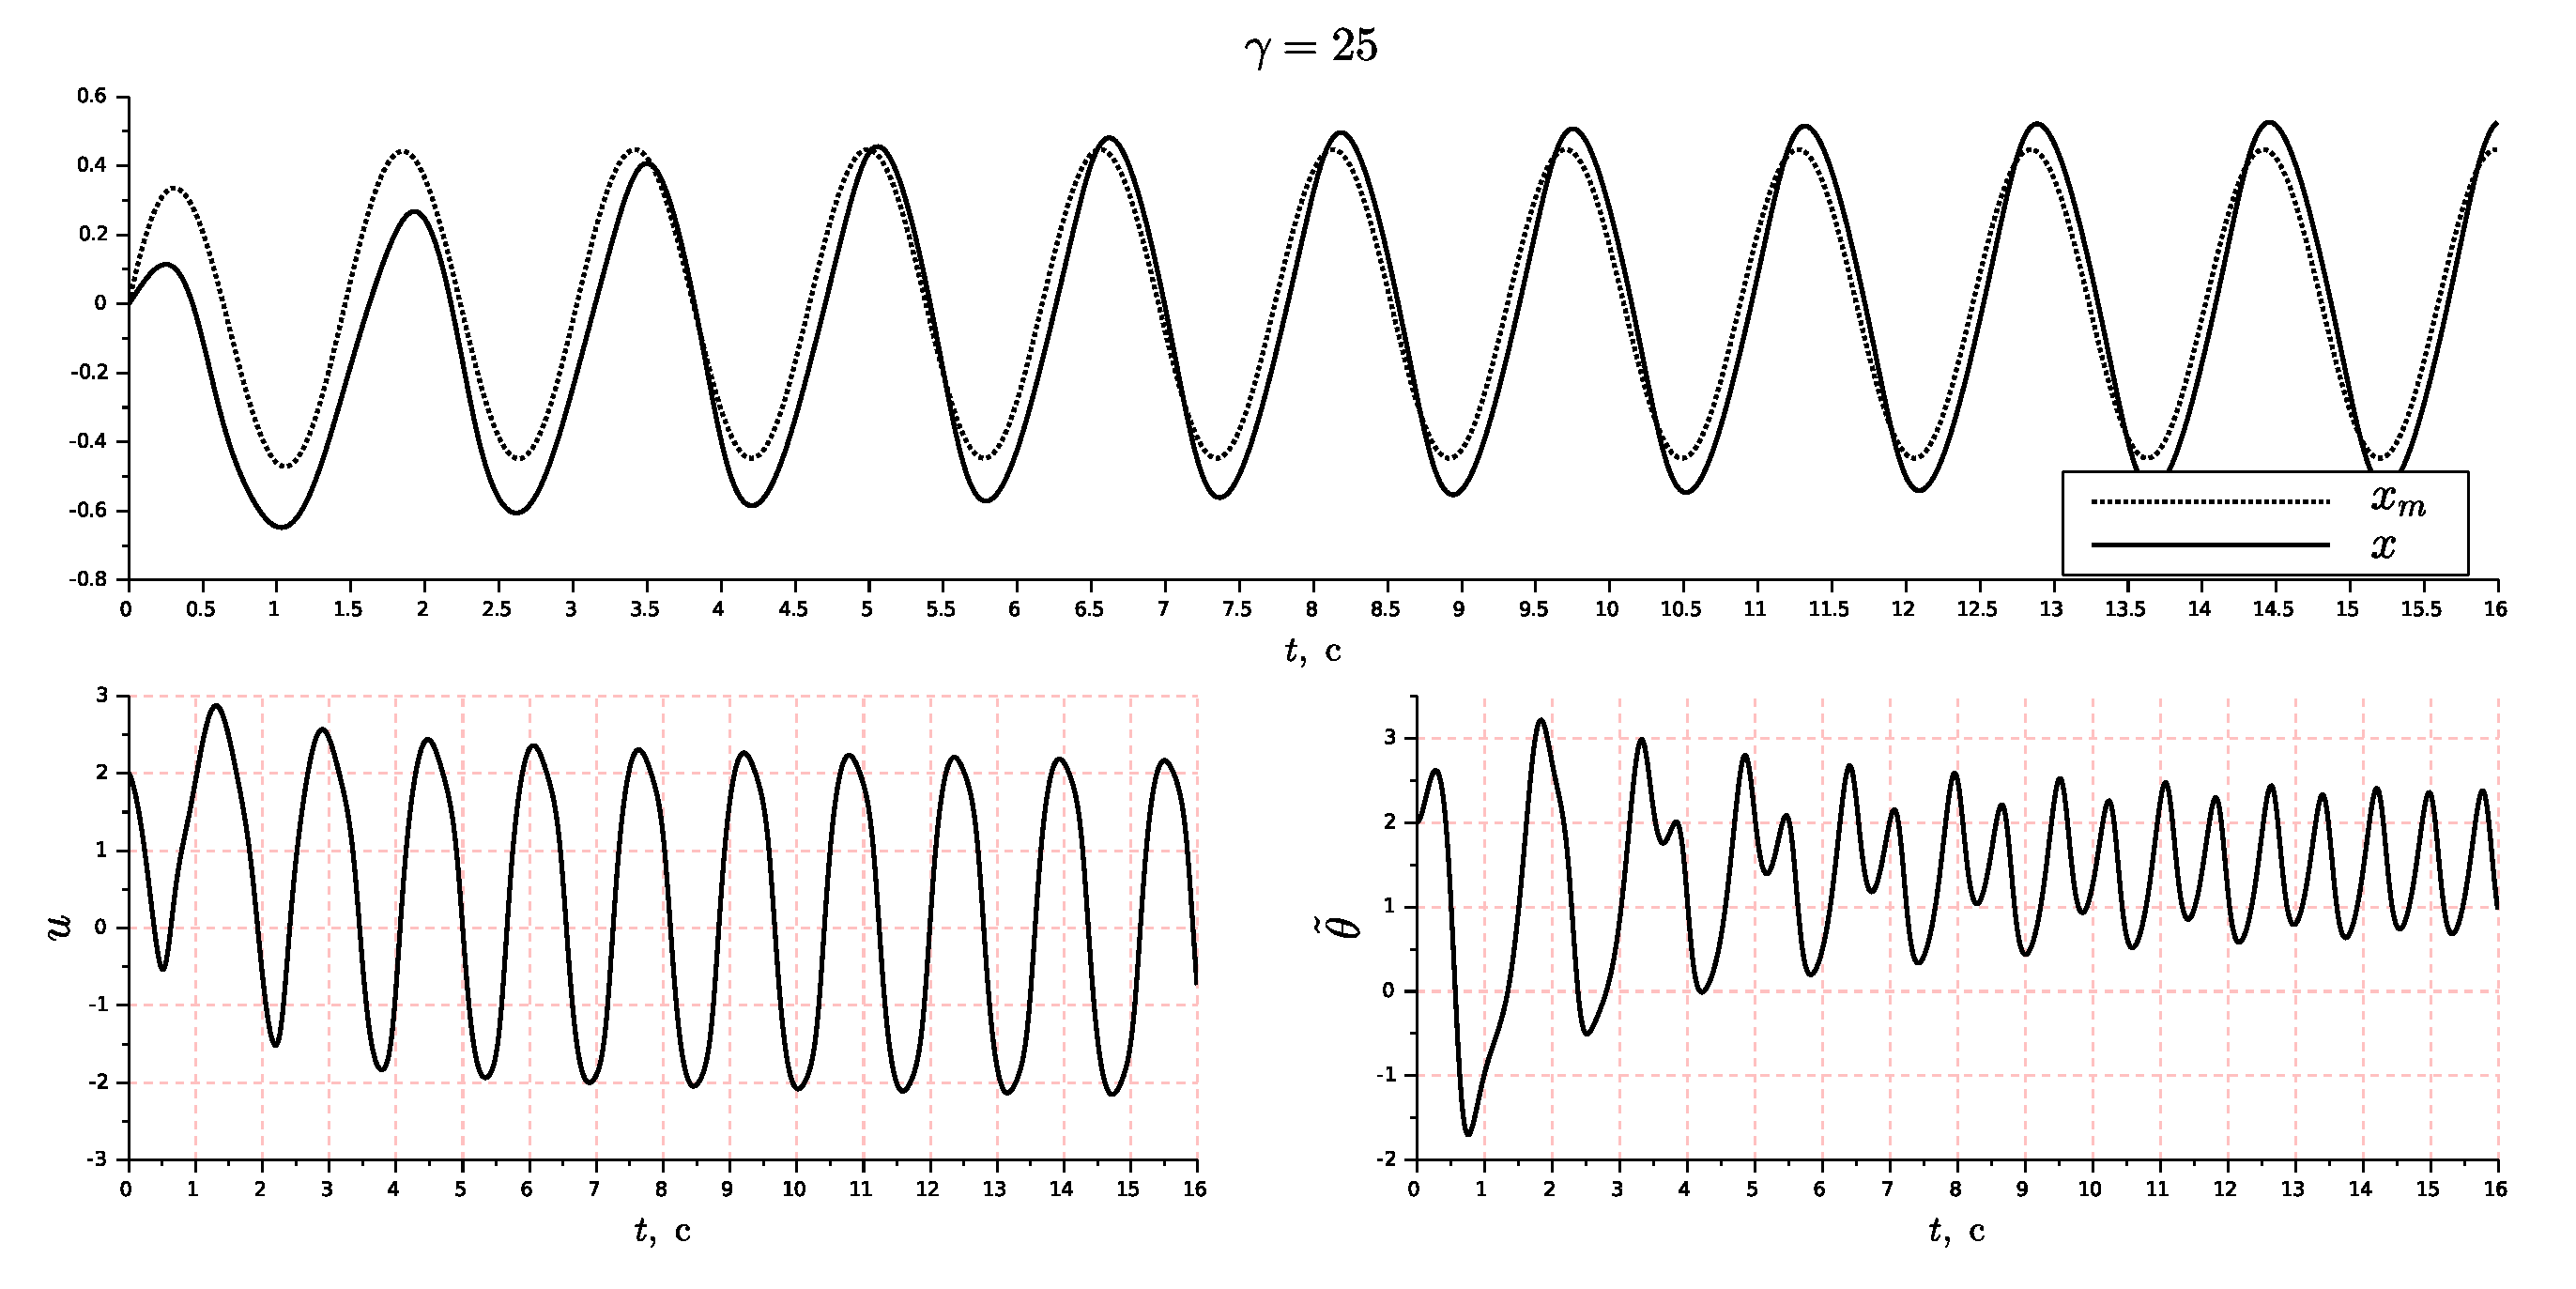
\includegraphics[width=\textwidth]{_adapt_desturbance_solve_1_g25.pdf}
    \caption{Результаты моделирования процесса управления с помощью настраиваемого регулятора с АА из п.2}
    \label{img_aa_2_g25}
\end{figure}

\begin{figure}[h!]
	\centering
	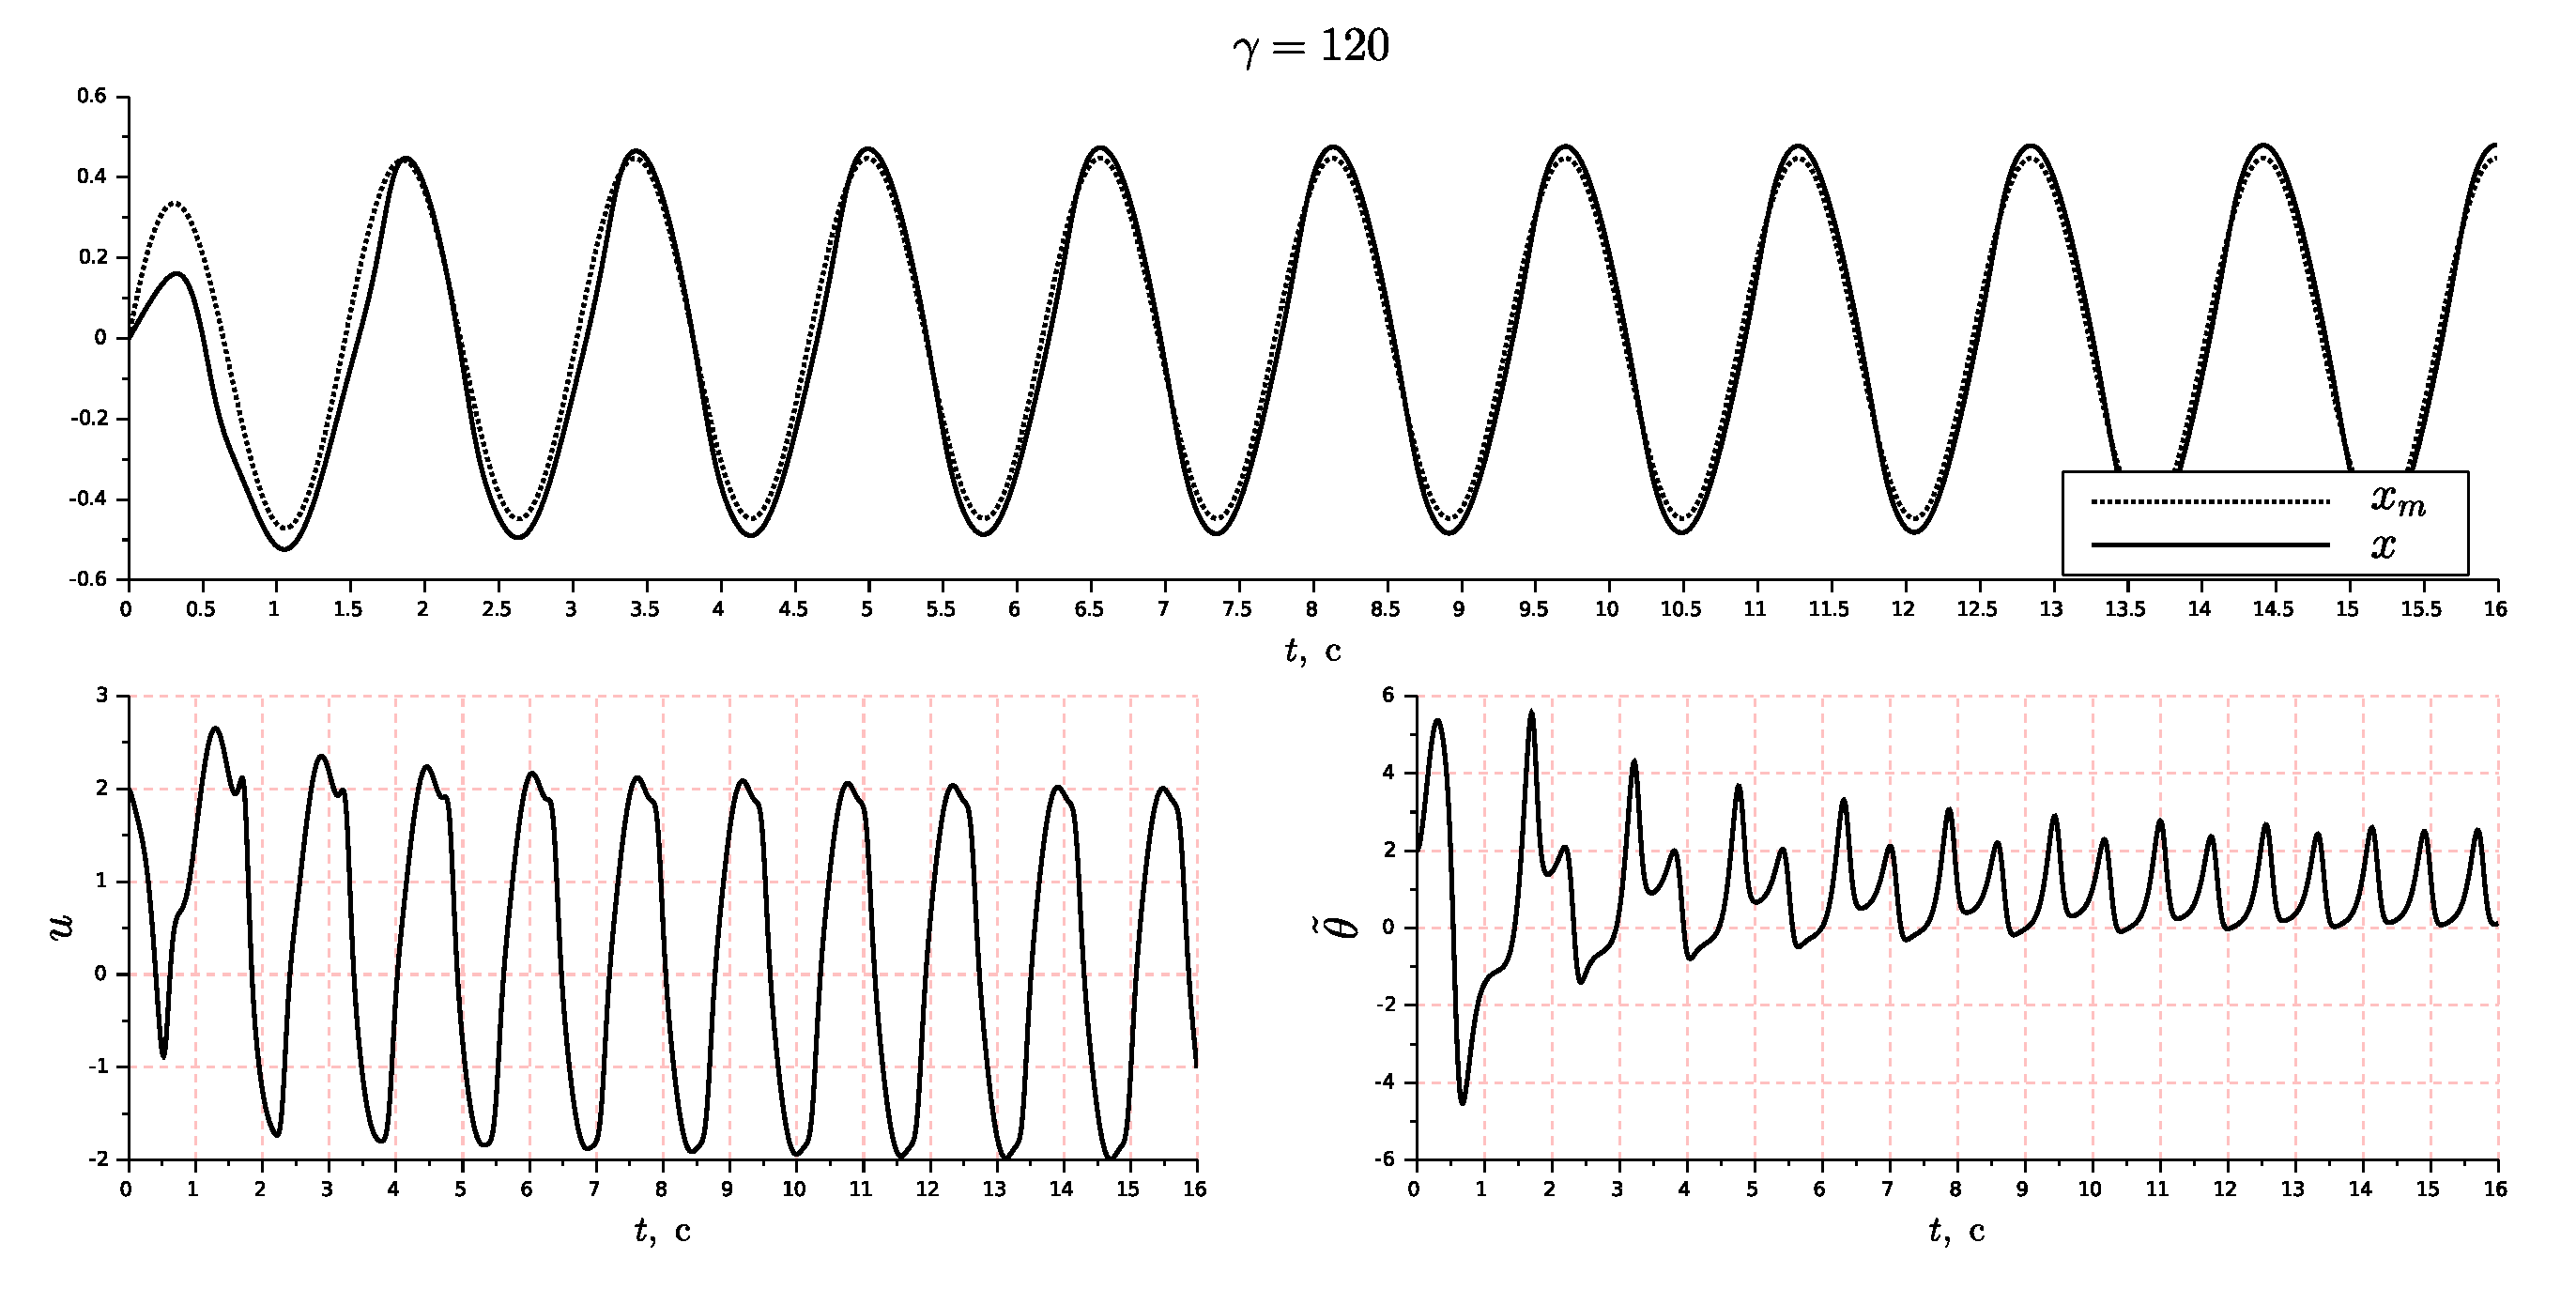
\includegraphics[width=\textwidth]{_adapt_desturbance_solve_1_g120.pdf}
	\caption{Результаты моделирования процесса управления с помощью настраиваемого регулятора с АА из п.2}
	\label{img_aa_2_g120}
\end{figure}

\begin{figure}[h!]
	\centering
	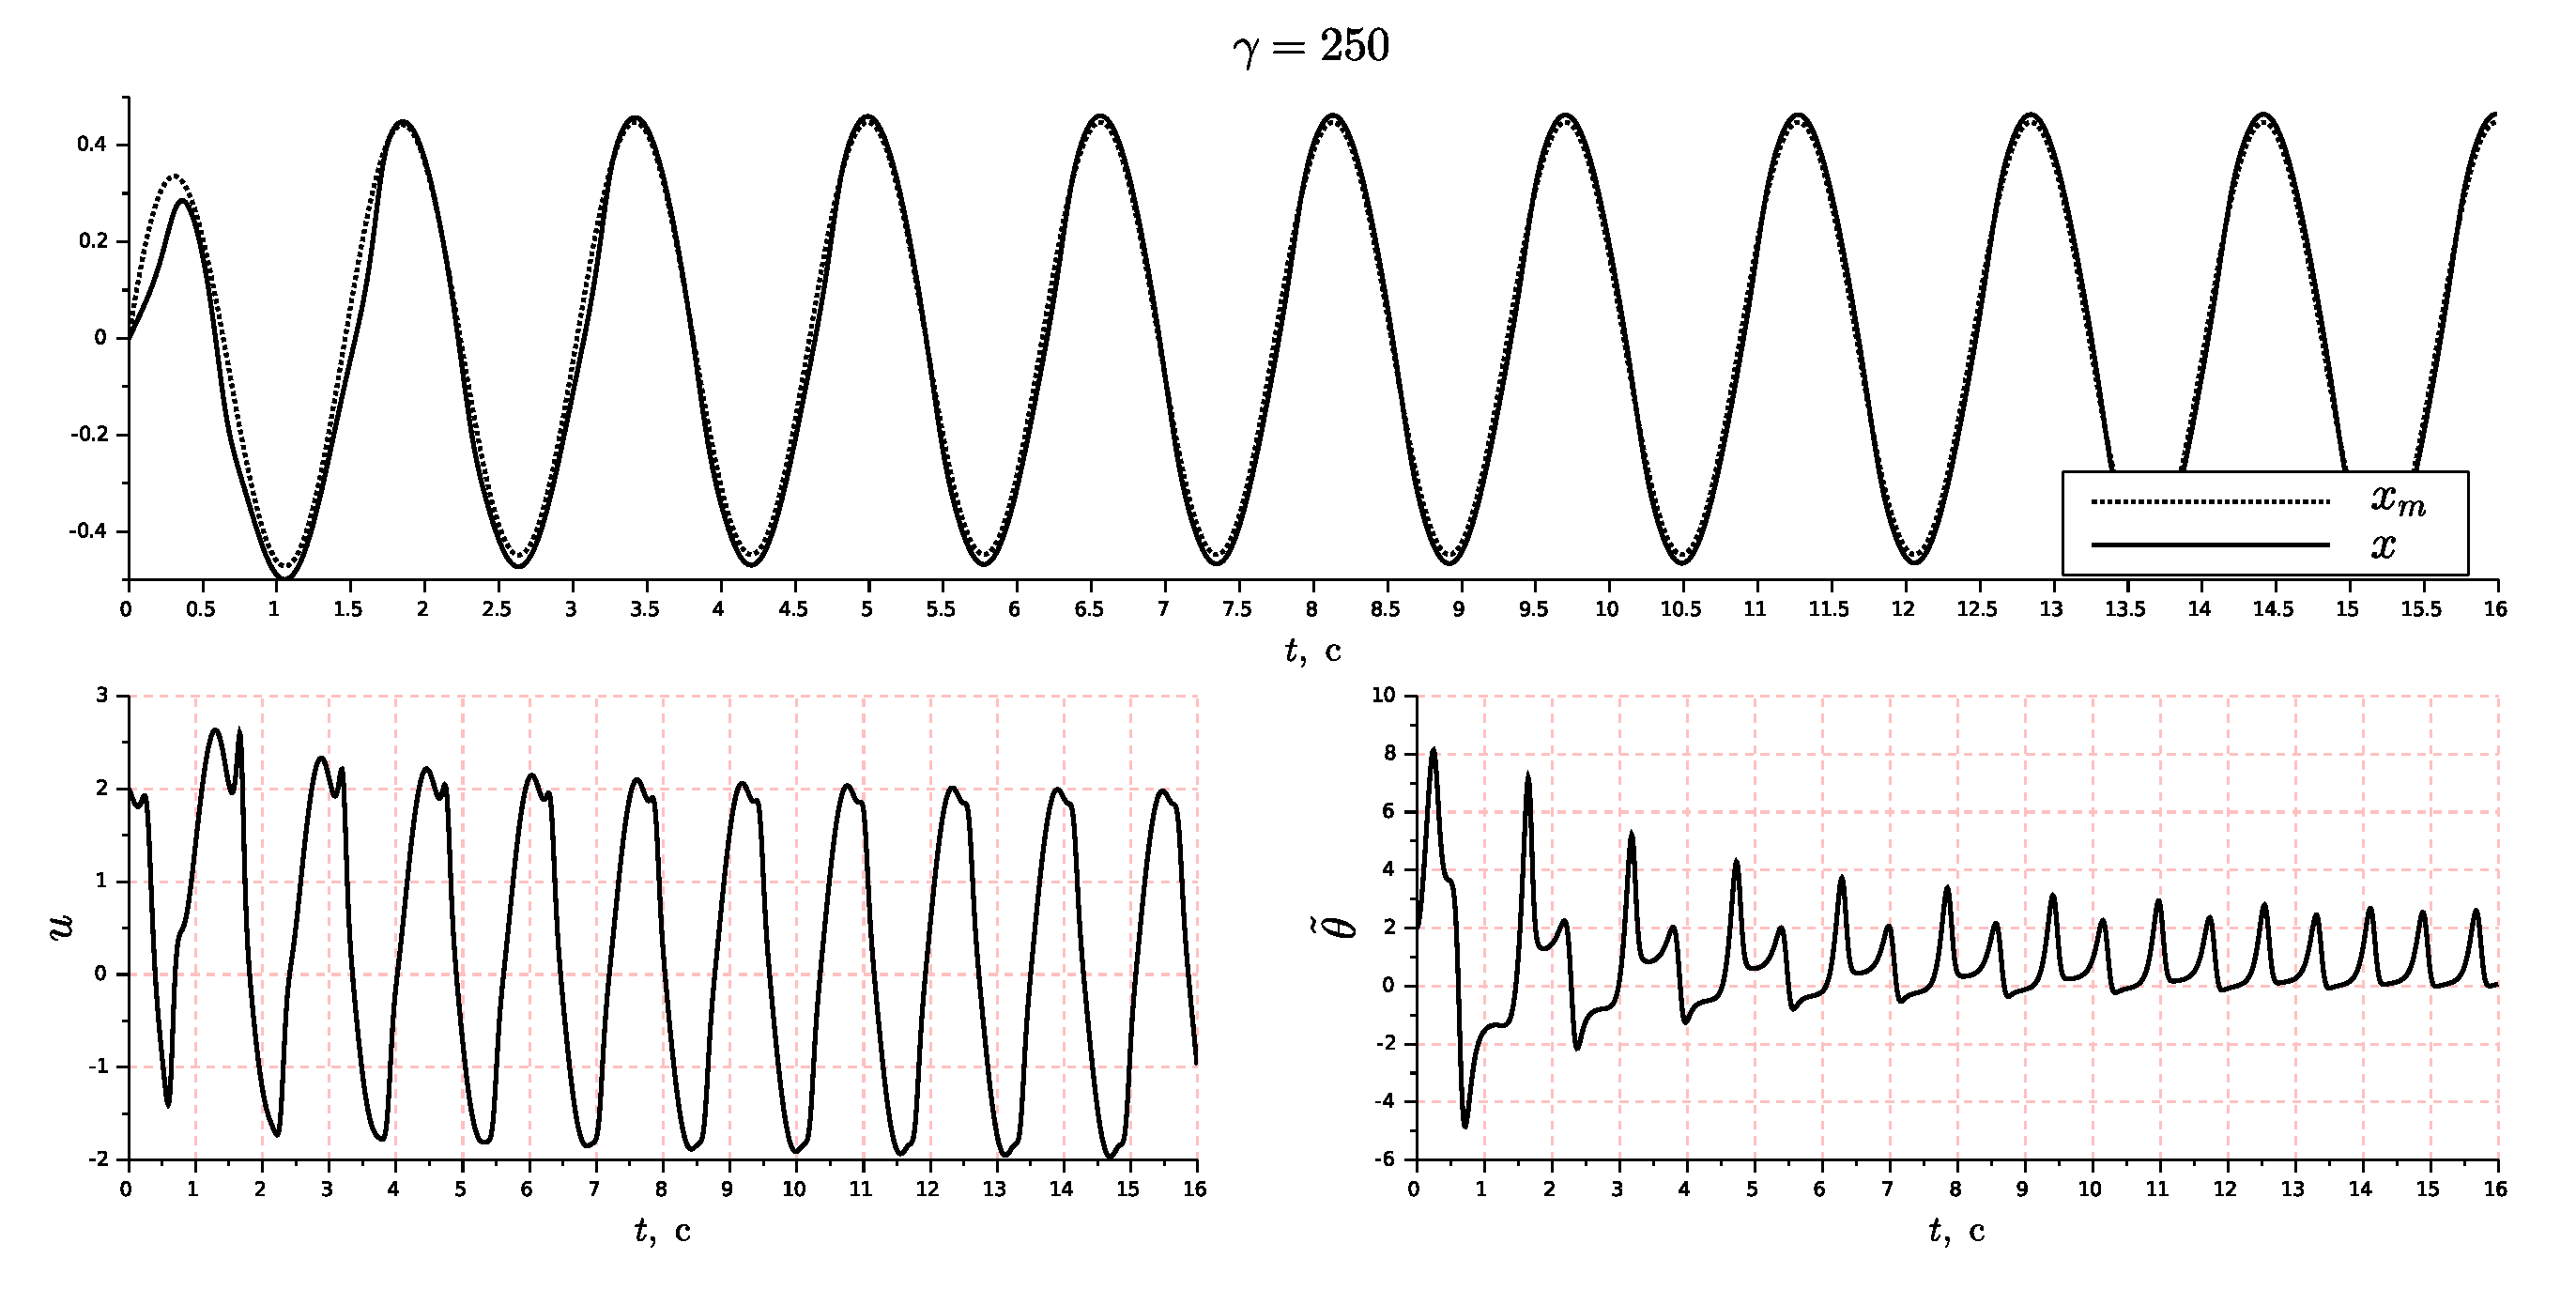
\includegraphics[width=\textwidth]{_adapt_desturbance_solve_1_g250.pdf}
	\caption{Результаты моделирования процесса управления с помощью настраиваемого регулятора с АА из п.2}
	\label{img_aa_2_g250}
\end{figure}

\begin{figure}[h!]
	\centering
	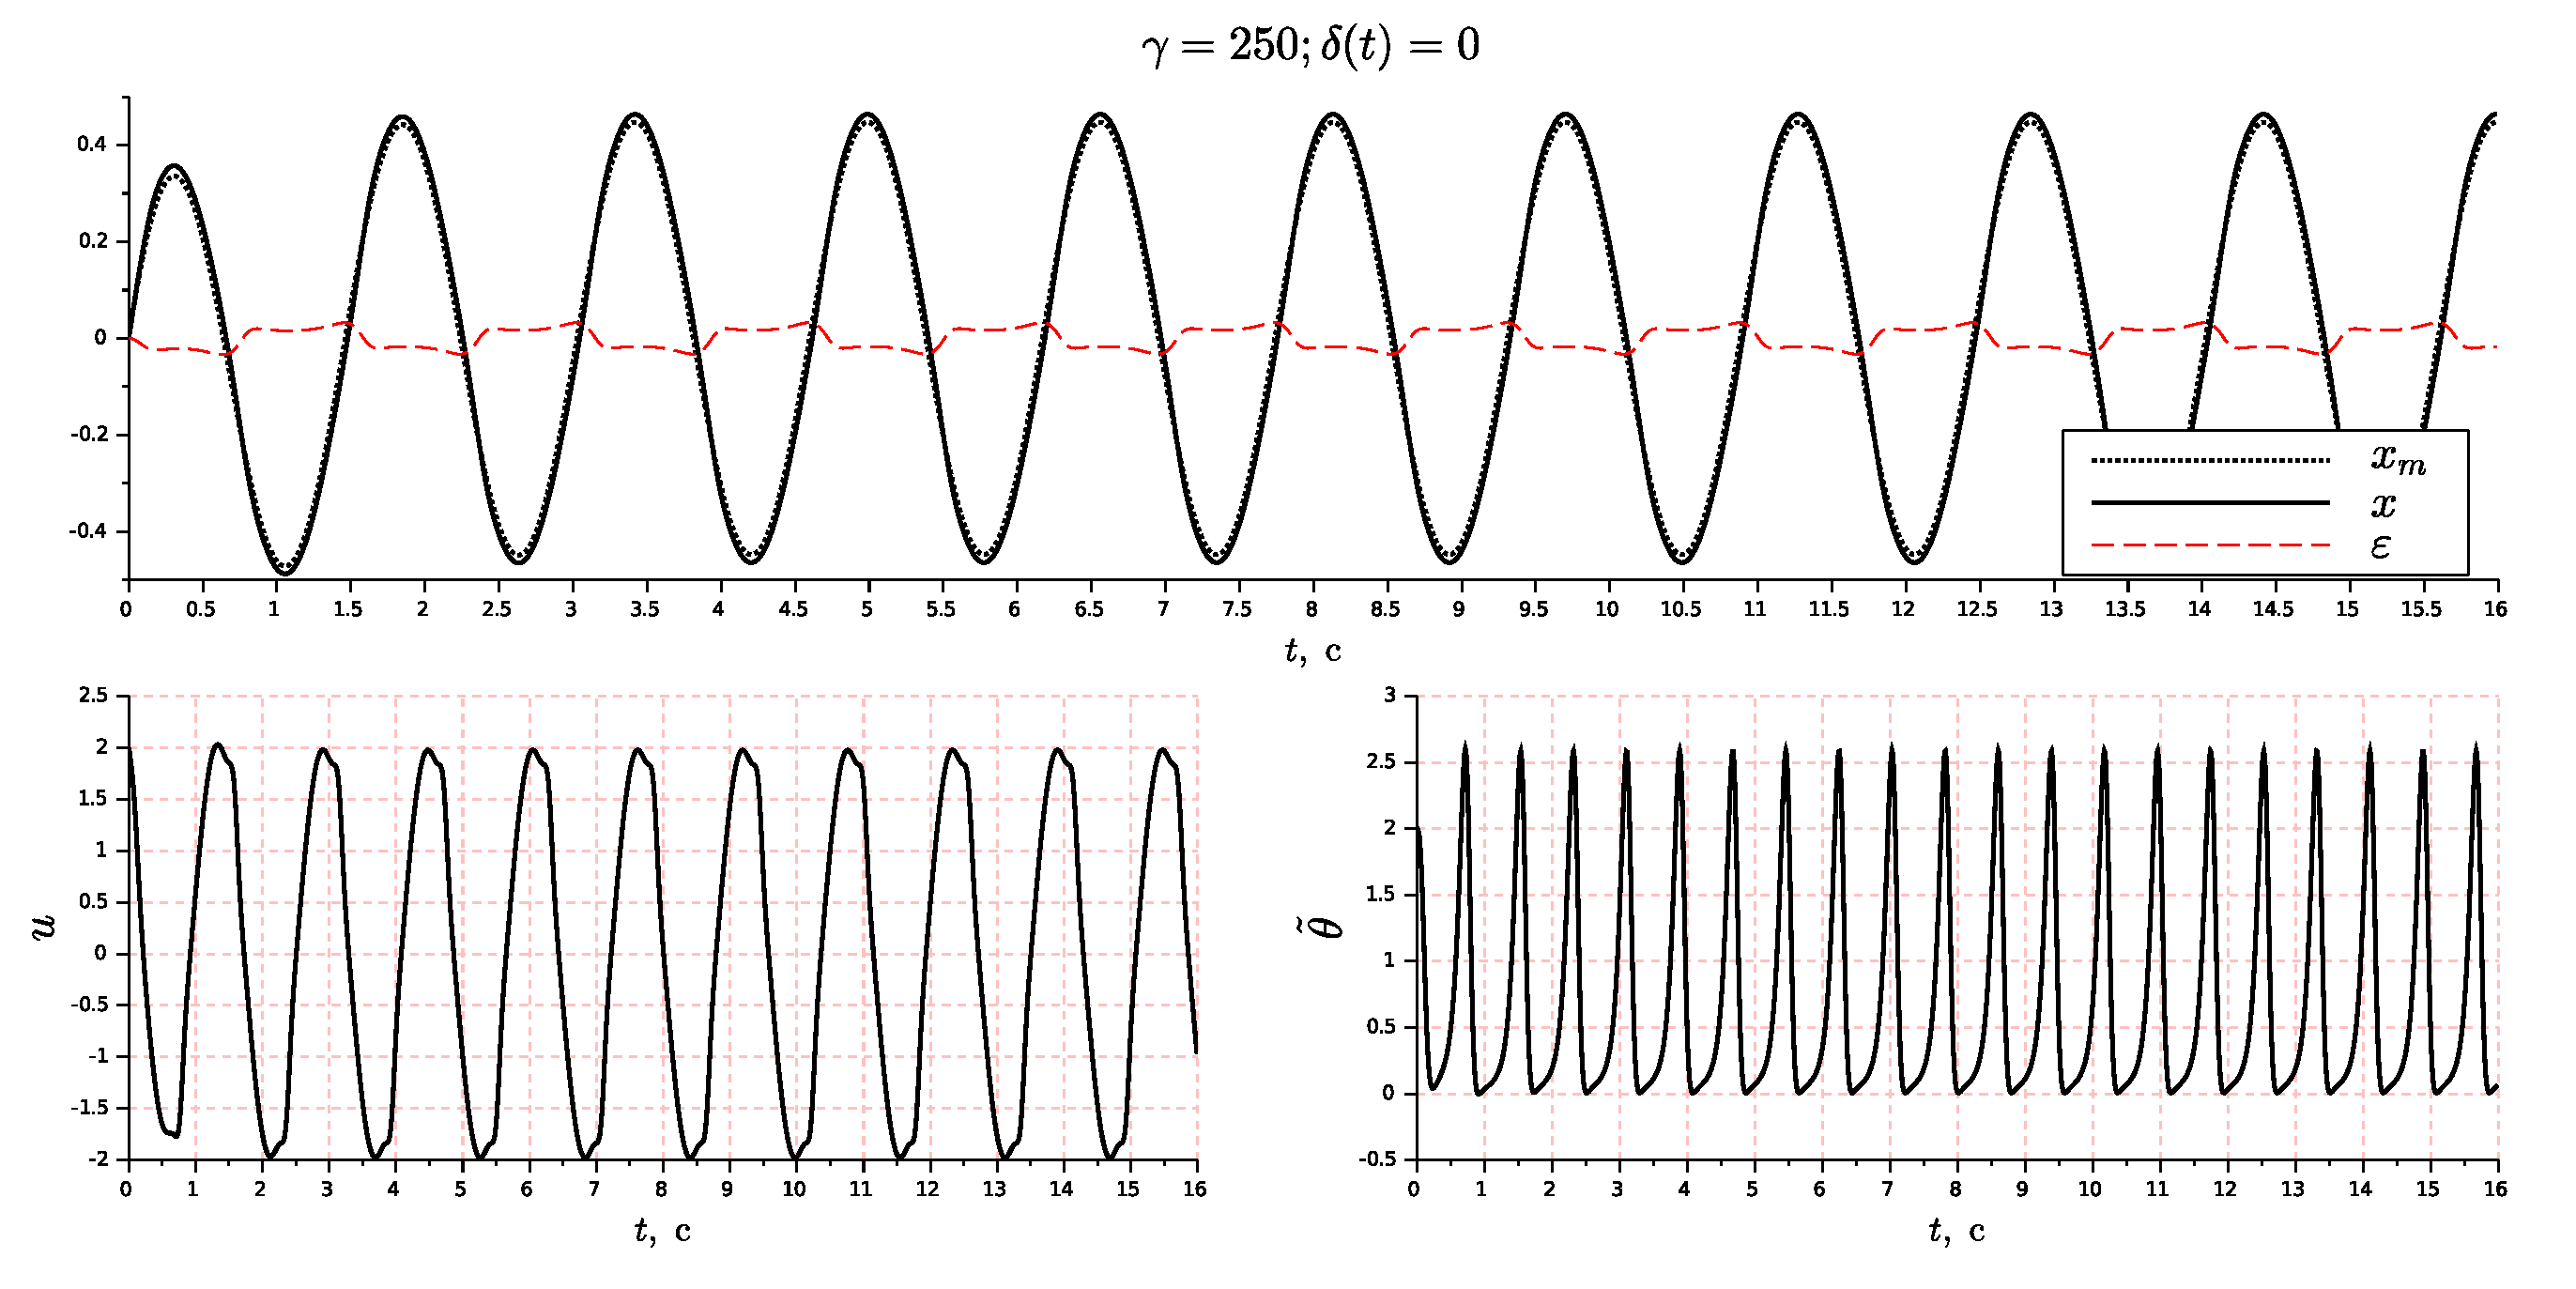
\includegraphics[width=\textwidth]{_adapt_NOdesturbance_solve_1_g250.pdf}
	\caption{Результаты моделирования процесса управления с помощью настраиваемого регулятора с АА из п.2 при отсутствии возмущения}
	\label{img_aa_2_g250_nodesturbance}
\end{figure}

\begin{figure}[h!]
	\centering
	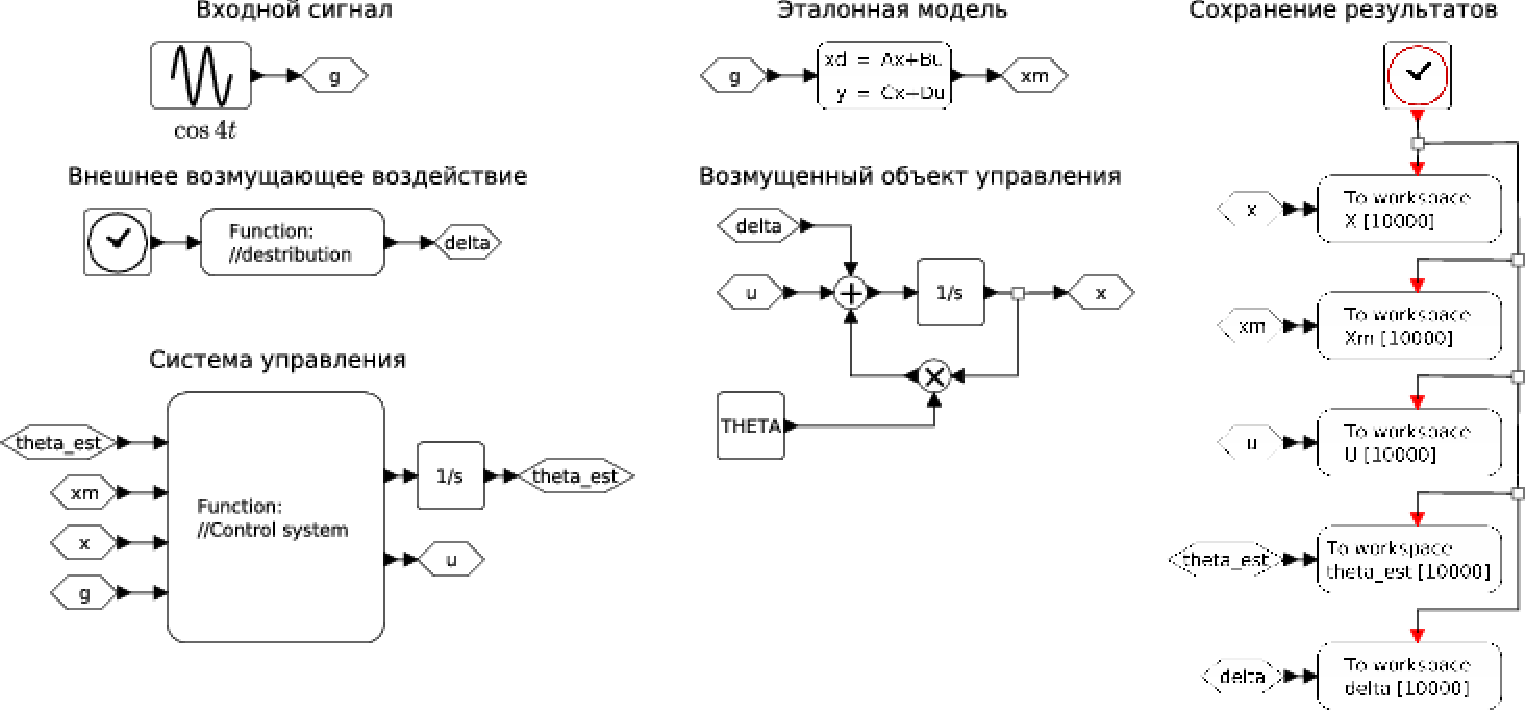
\includegraphics[width=\textwidth]{adapt_desturbance_model_solve_2.pdf}
	\caption{Схема моделирования процесса управления с помощью настраиваемого регулятора из п.3 в условиях действия на ОУ возмущения~\ref{eq_delta}}
	\label{img_schema_3}
\end{figure}

\begin{figure}[h!]
	\centering
	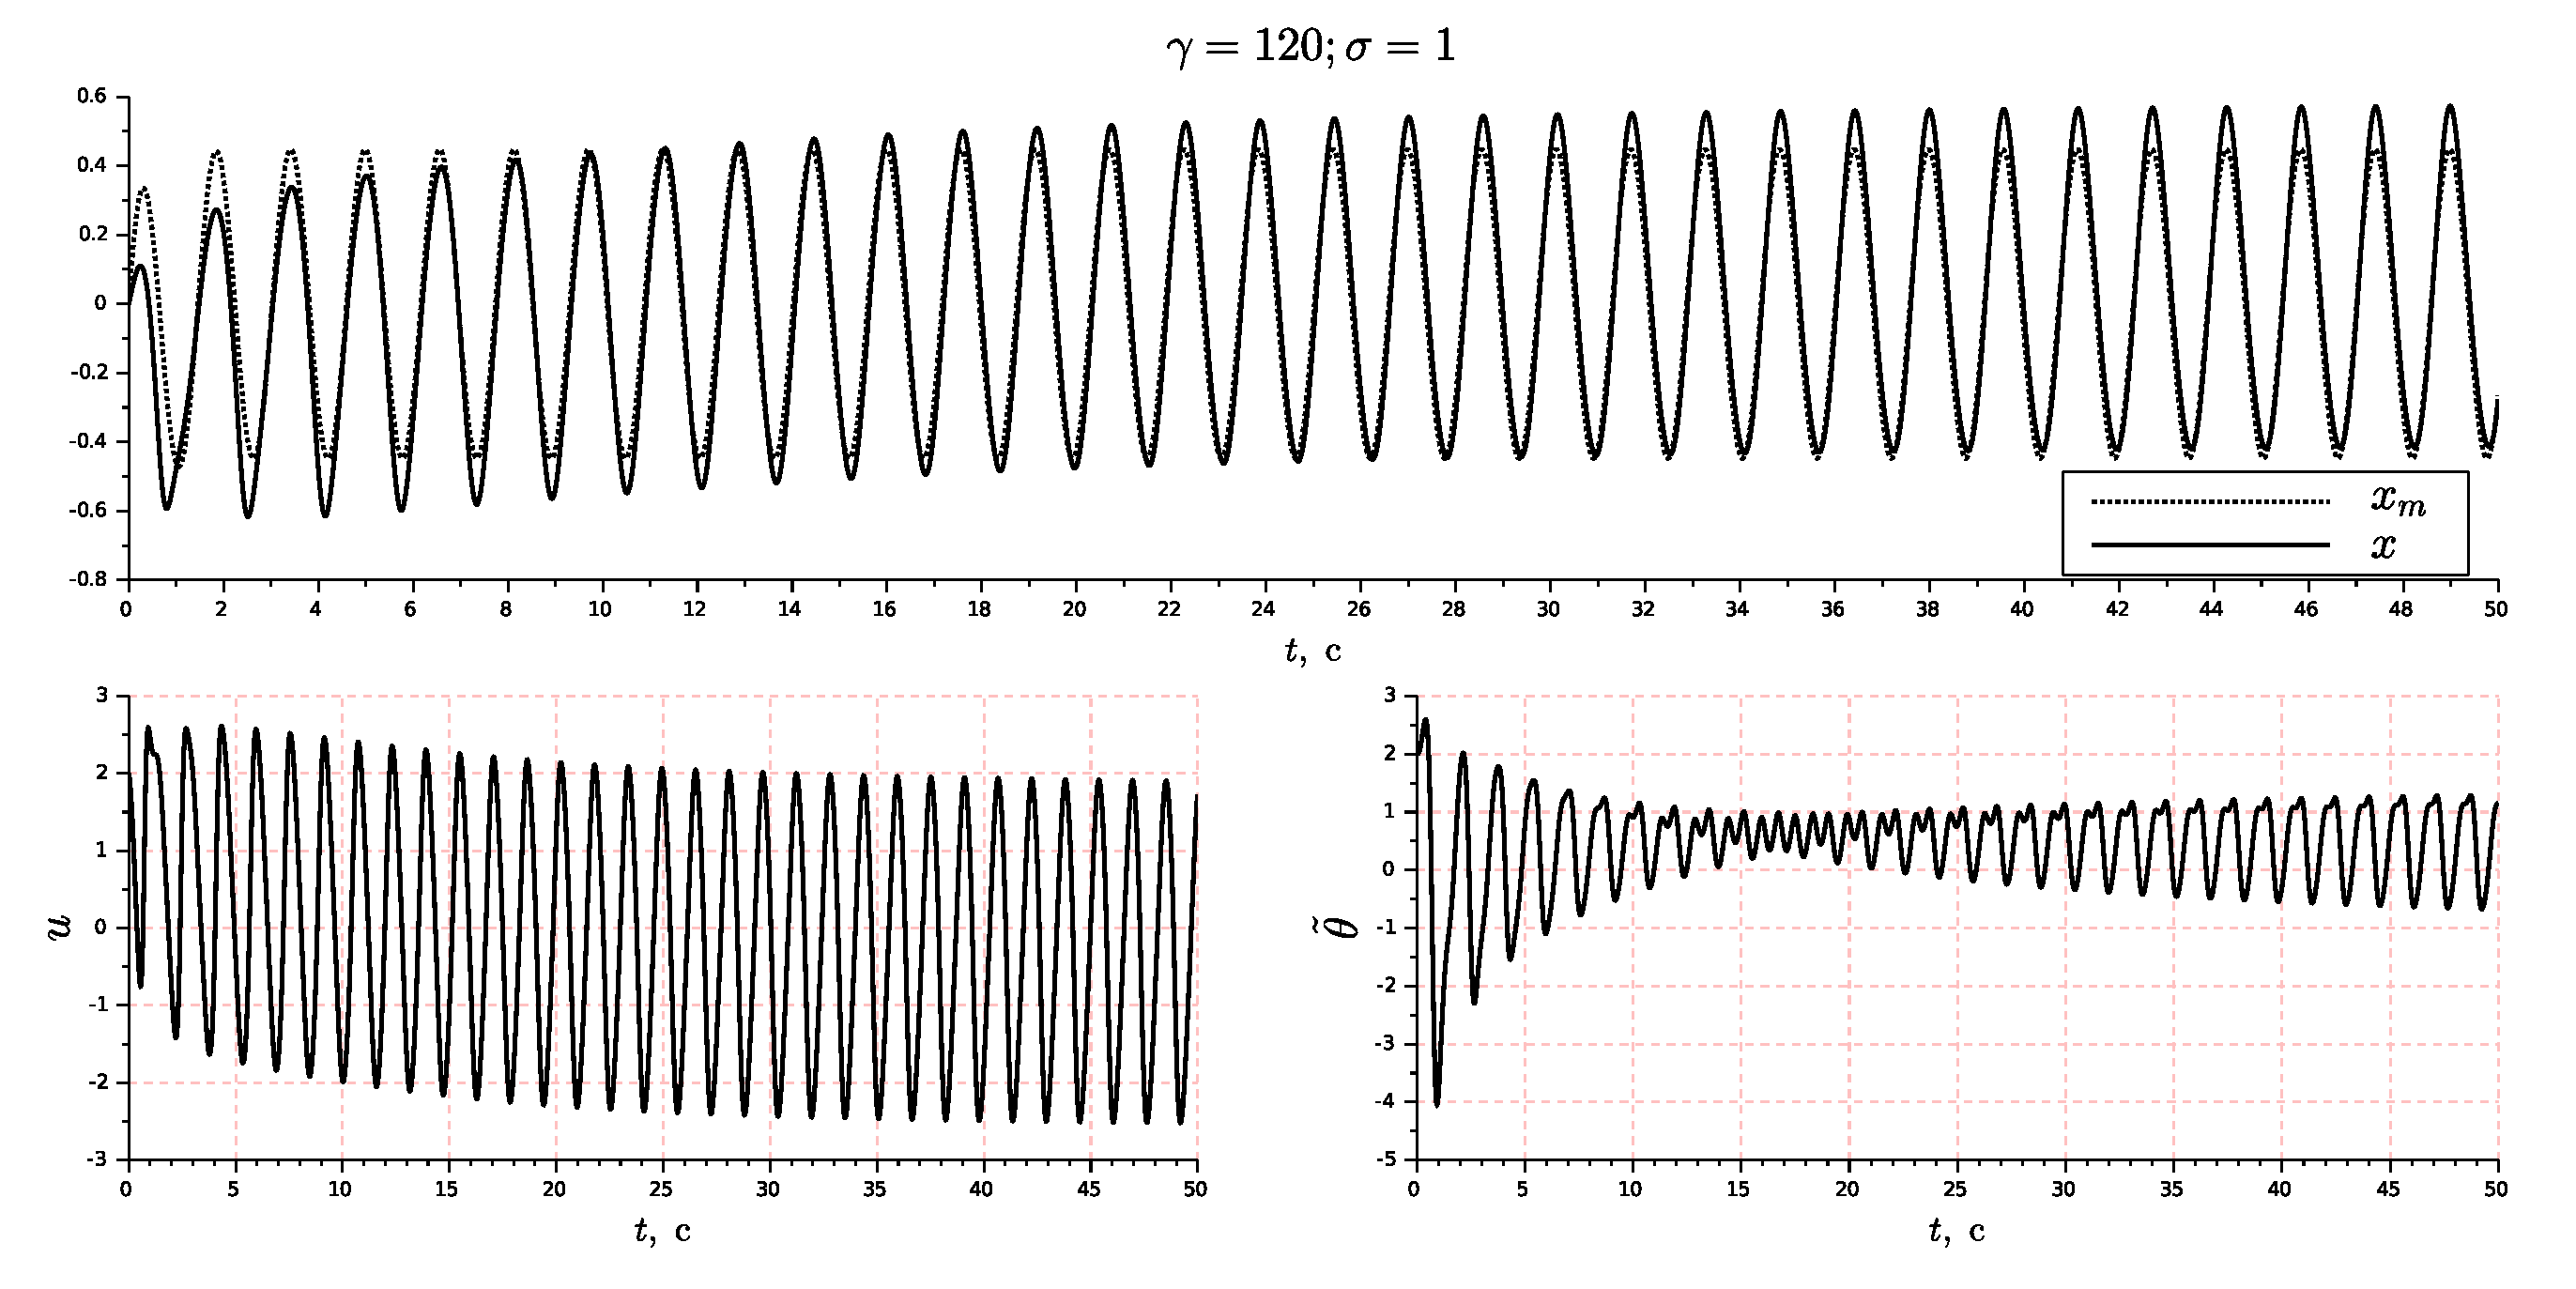
\includegraphics[width=\textwidth]{_adapt_desturbance_solve_2_s1.pdf}
	\caption{Результаты моделирования процесса управления с помощью настраиваемого регулятора с АА из п.3}
	\label{img_aa_3_s1}
\end{figure}

\begin{figure}[h!]
	\centering
	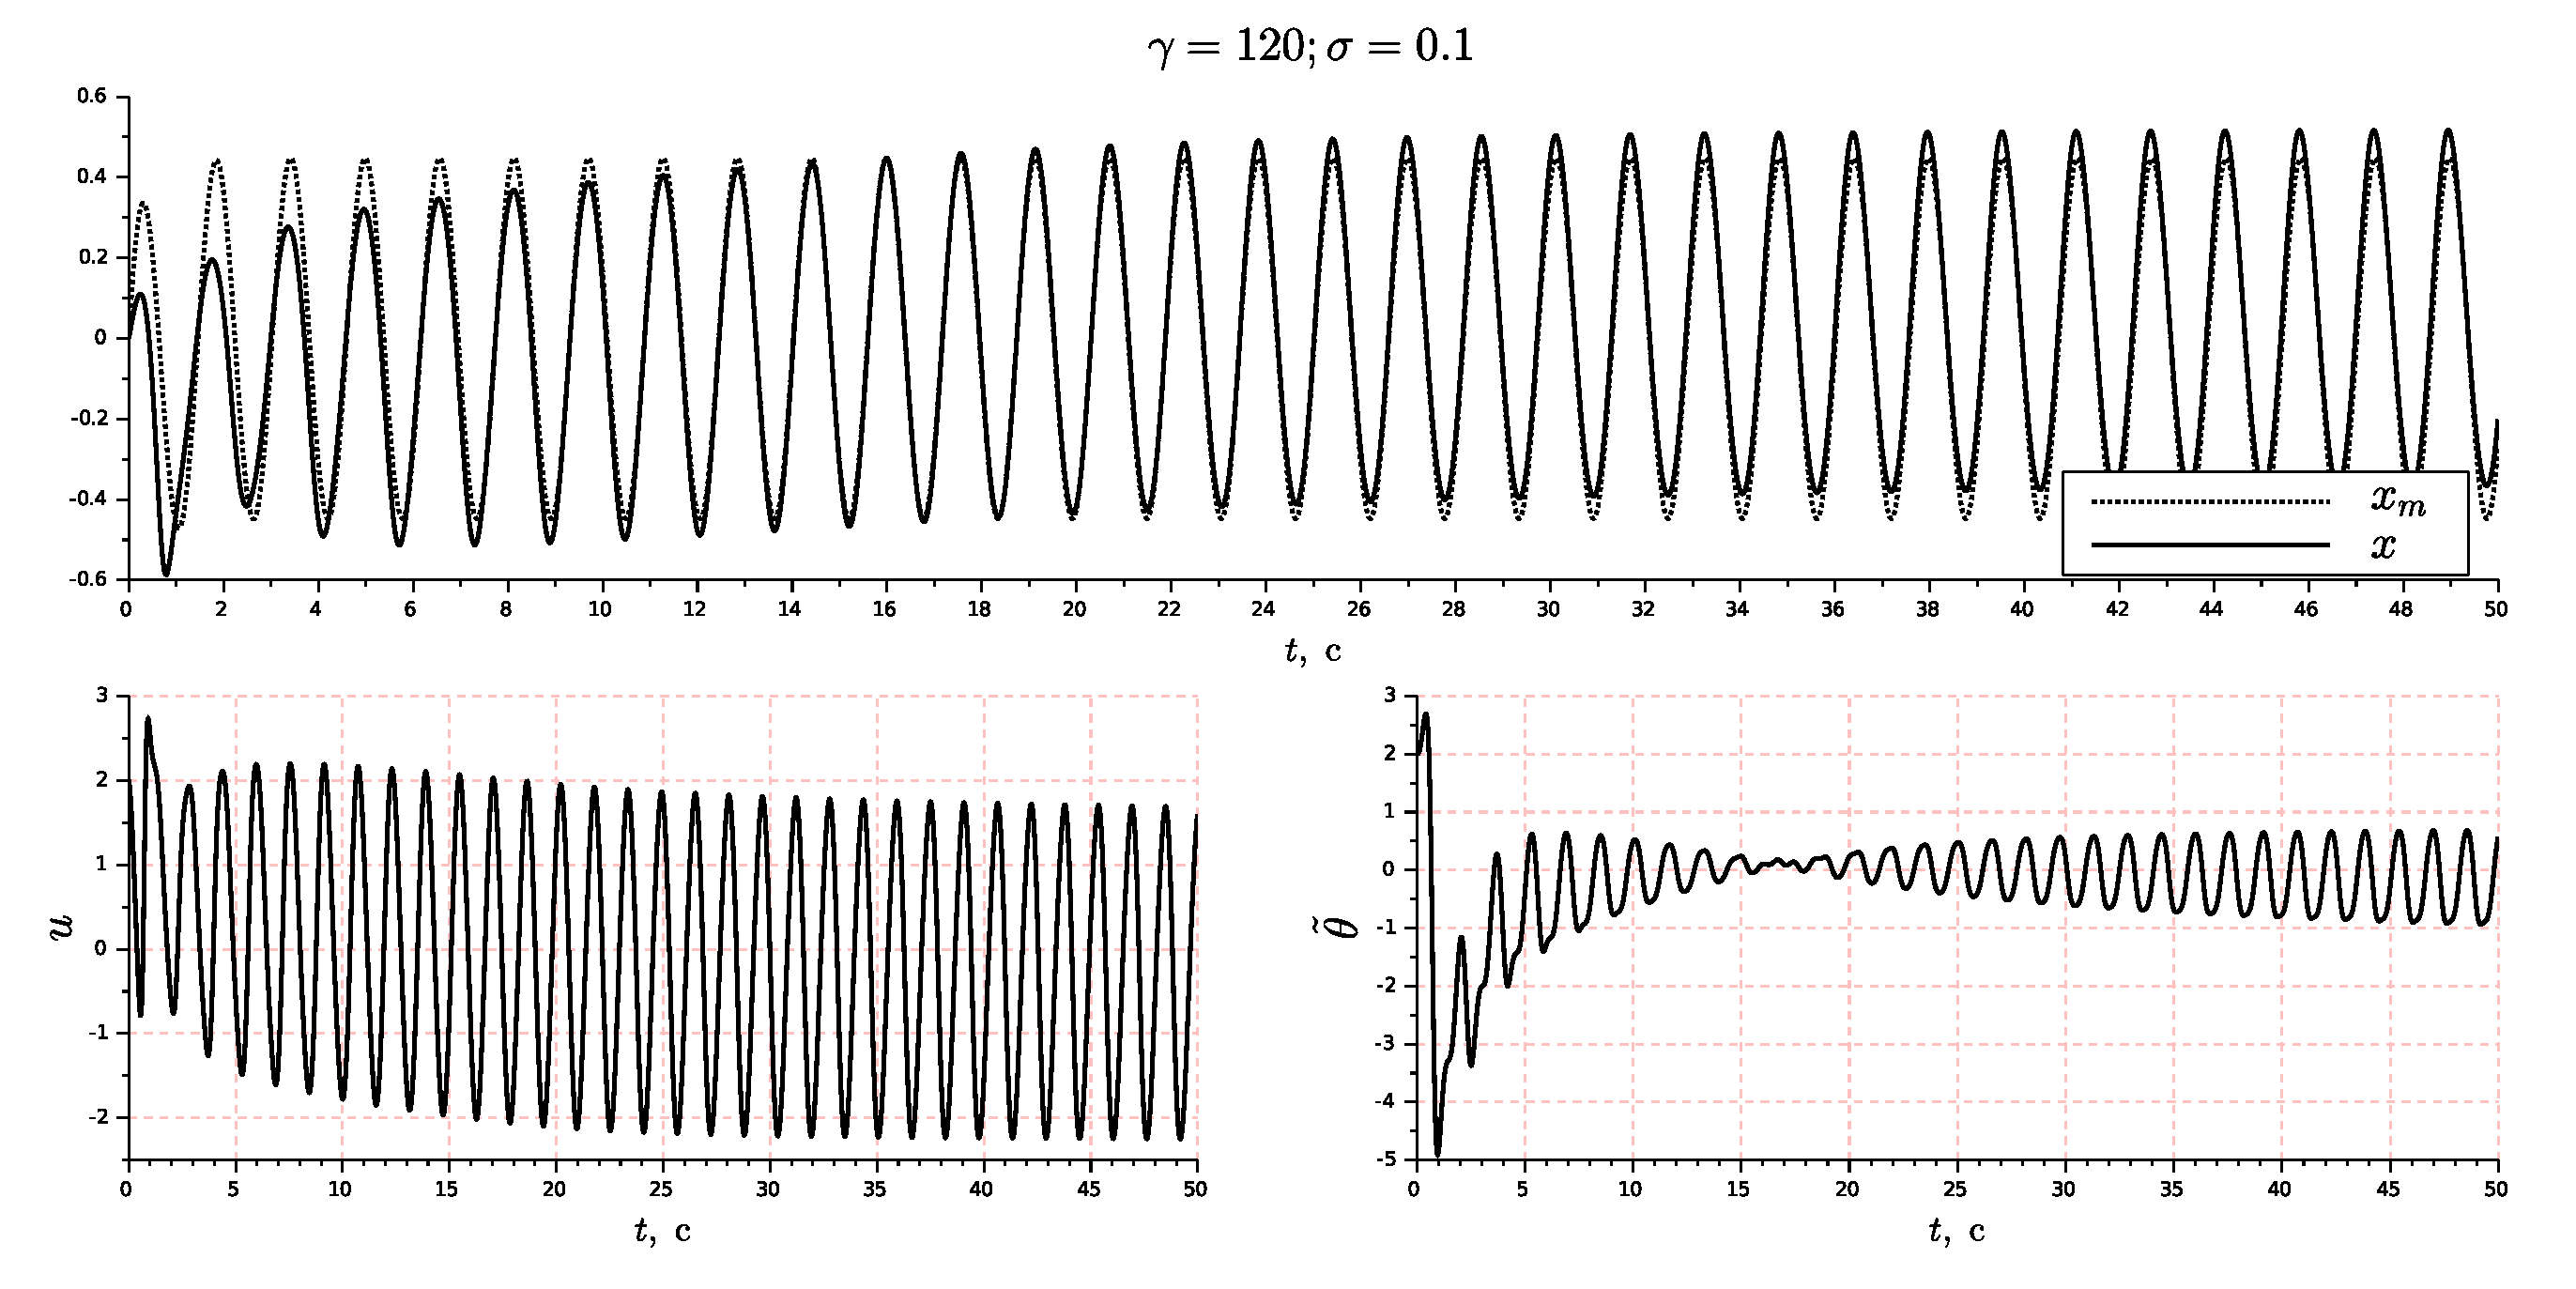
\includegraphics[width=\textwidth]{_adapt_desturbance_solve_2_s01.pdf}
	\caption{Результаты моделирования процесса управления с помощью настраиваемого регулятора с АА из п.3}
	\label{img_aa_3_s0.1}
\end{figure}

\begin{figure}[h!]
	\centering
	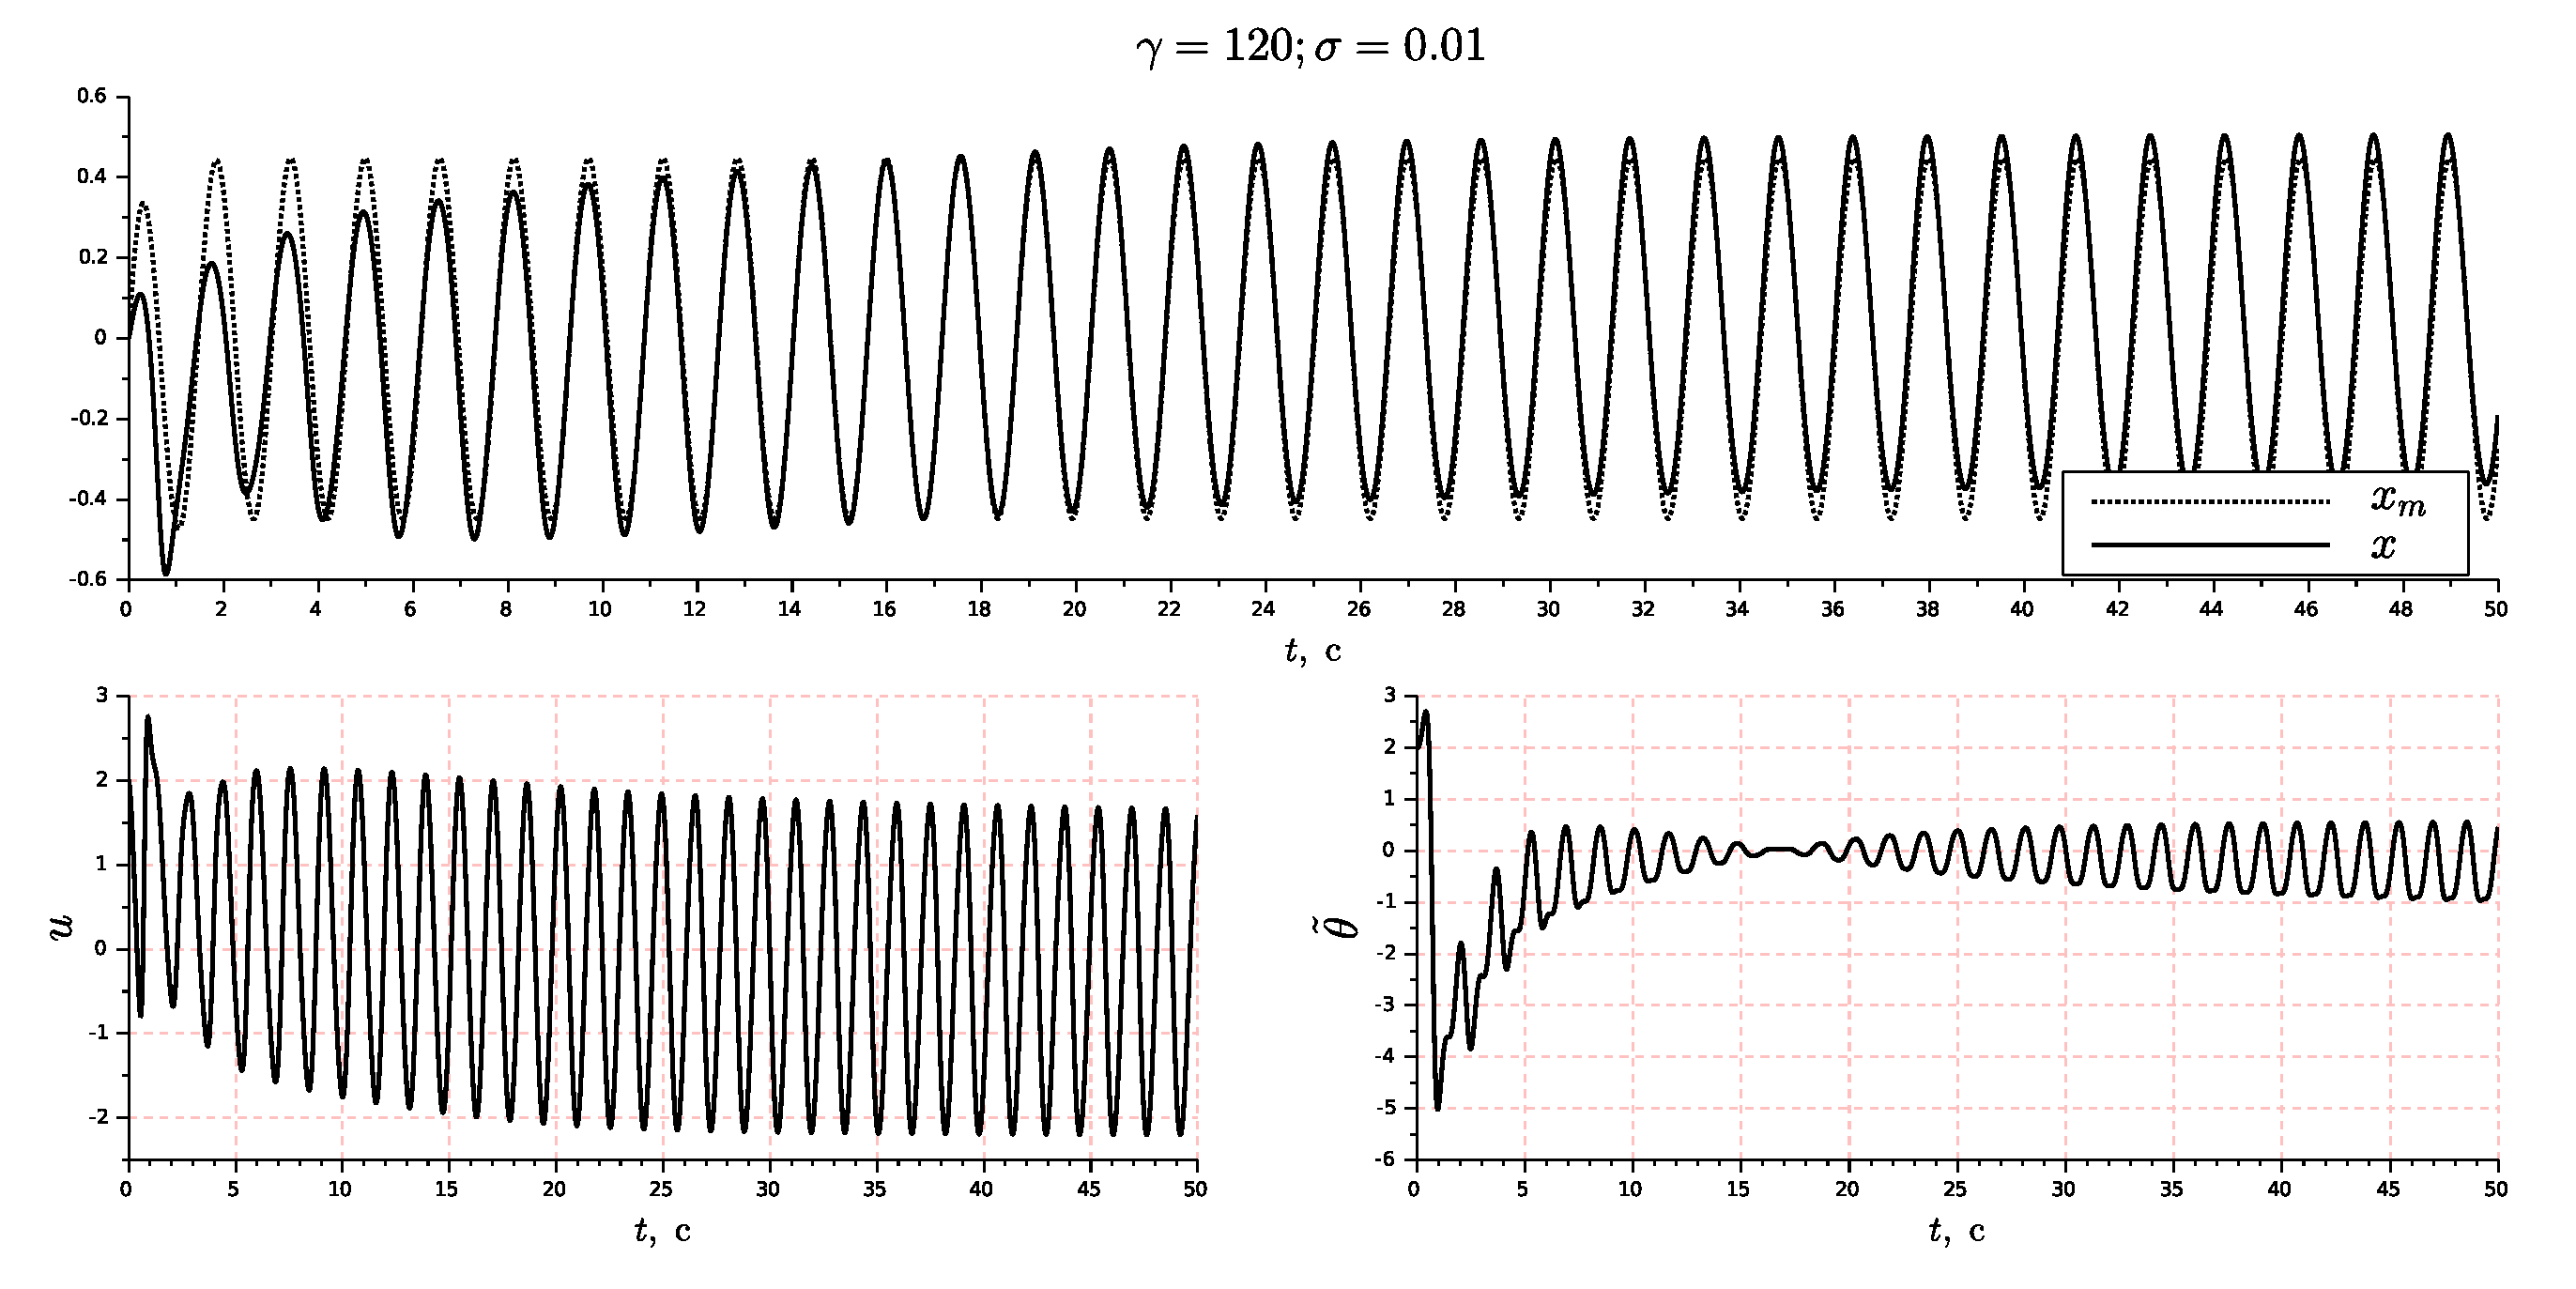
\includegraphics[width=\textwidth]{_adapt_desturbance_solve_2_s001.pdf}
	\caption{Результаты моделирования процесса управления с помощью настраиваемого регулятора с АА из п.3}
	\label{img_aa_3_s0.01}
\end{figure}


\newpage
\mbox{}
\newpage

\clearpage
\section{Выводы по работе}
В~результате проделанной работы экспериментальным путем было установлено, что
\begin{itemize}
	\item настраиваемый регулятор с АА~\eqref{eq_AA_1} обеспечивает устойчивость замкнутой системы, но в общем случае не обеспечивает ограниченности оценки параметра при наличии ограниченного внешнего возмущения~\ref{img_aa_1};
	\item настраиваемый регулятор с АА~\eqref{eq_AA_2} добавляет системе свойства робастности по отношению к внешнему воздействию, но увеличивает амплитуду управляющего воздействия до $x^2$ и не позволяет избавиться от ненулевой установившейся ошибки даже при отсутствии внешнего возмущения. Увеличение значения коэффициента адаптации увеличивает скорость (время) сходимости оценки $\hat{\theta}$ к истинному значению параметра $\theta$ ОУ и точность системы, но увеличивает амплитуду управляющего сигнала;
	\item настраиваемый регулятор с АА~\eqref{eq_AA_3} обеспечивает устойчивость замкнутой системы и является робастным по отношению к внешнему возмущению. В то же время позволяет парировать недостатки робастного алгоритма управления. Так, при отсутствии внешнего возмущения точность системы может быть увеличена засчет уменьшения коэффициента $\sigma$.
\end{itemize}